
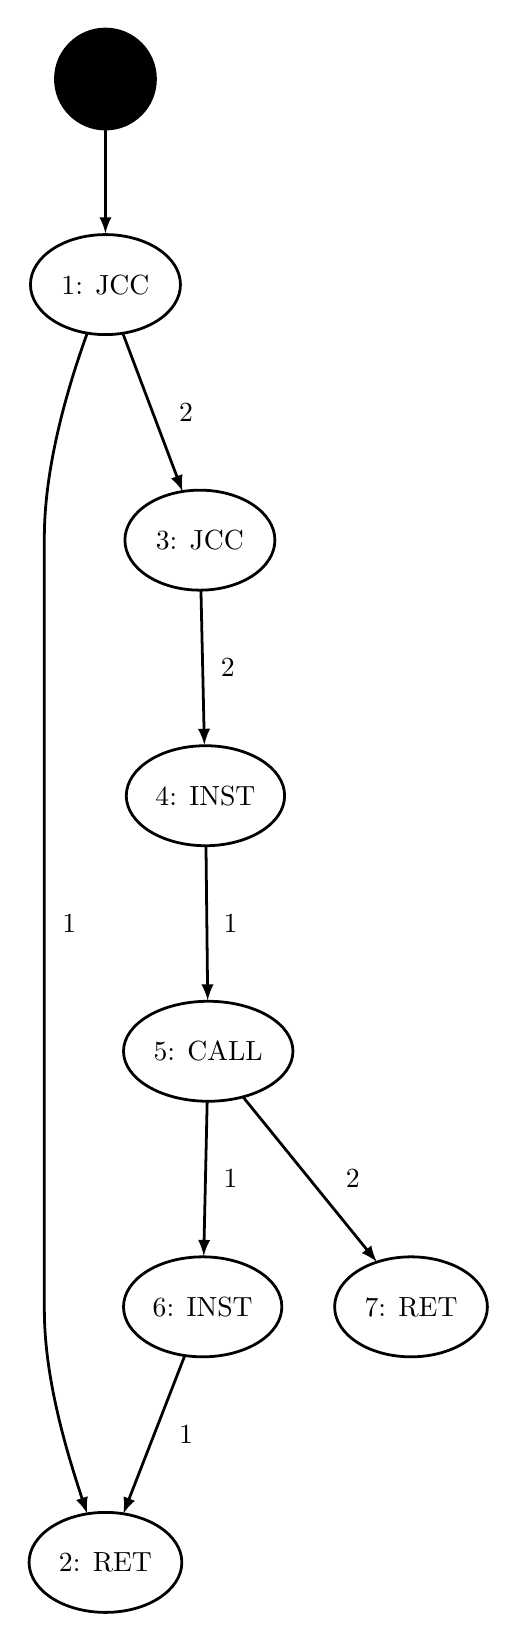
\begin{tikzpicture}[>=latex,line join=bevel,]
  \pgfsetlinewidth{1bp}
%%
\pgfsetcolor{black}
  % Edge: 2 -> 3
  \draw [->] (63.614bp,183.65bp) .. controls (63.329bp,170.82bp) and (62.936bp,153.11bp)  .. (62.384bp,128.3bp);
  \definecolor{strokecol}{rgb}{0.0,0.0,0.0};
  \pgfsetstrokecolor{strokecol}
  \draw (72.0bp,156.0bp) node {1};
  % Edge: 6 -> 7
  \draw [->] (61.386bp,367.65bp) .. controls (61.671bp,354.82bp) and (62.064bp,337.11bp)  .. (62.616bp,312.3bp);
  \draw (71.0bp,340.0bp) node {2};
  % Edge: 1 -> 6
  \draw [->] (33.395bp,460.07bp) .. controls (38.413bp,446.79bp) and (45.484bp,428.07bp)  .. (54.748bp,403.55bp);
  \draw (56.0bp,432.0bp) node {2};
  % Edge: 7 -> 2
  \draw [->] (63.193bp,275.65bp) .. controls (63.335bp,262.82bp) and (63.532bp,245.11bp)  .. (63.808bp,220.3bp);
  \draw (72.0bp,248.0bp) node {1};
  % Edge: 1 -> 4
  \draw [->] (20.399bp,460.38bp) .. controls (13.919bp,442.54bp) and (5.0bp,413.22bp)  .. (5.0bp,387.0bp) .. controls (5.0bp,387.0bp) and (5.0bp,387.0bp)  .. (5.0bp,109.0bp) .. controls (5.0bp,87.083bp) and (11.233bp,63.0bp)  .. (20.399bp,35.622bp);
  \draw (14.0bp,248.0bp) node {1};
  % Edge: 0 -> 1
  \draw [->] (27.0bp,533.94bp) .. controls (27.0bp,525.81bp) and (27.0bp,515.88bp)  .. (27.0bp,496.44bp);
  % Edge: 2 -> 5
  \draw [->] (76.716bp,185.32bp) .. controls (88.195bp,171.17bp) and (105.23bp,150.16bp)  .. (124.67bp,126.2bp);
  \draw (116.0bp,156.0bp) node {2};
  % Edge: 3 -> 4
  \draw [->] (55.417bp,92.072bp) .. controls (50.251bp,78.789bp) and (42.973bp,60.073bp)  .. (33.435bp,35.548bp);
  \draw (56.0bp,64.0bp) node {1};
  % Node: 1
\begin{scope}
  \definecolor{strokecol}{rgb}{0.0,0.0,0.0};
  \pgfsetstrokecolor{strokecol}
  \draw (27.0bp,478.0bp) ellipse (27.0bp and 18.0bp);
  \draw (27.0bp,478.0bp) node {1: JCC};
\end{scope}
  % Node: 0
\begin{scope}
  \definecolor{strokecol}{rgb}{0.0,0.0,0.0};
  \pgfsetstrokecolor{strokecol}
  \definecolor{fillcol}{rgb}{0.0,0.0,0.0};
  \pgfsetfillcolor{fillcol}
  \filldraw [opacity=1] (27.0bp,552.0bp) ellipse (18.0bp and 18.0bp);
\end{scope}
  % Node: 3
\begin{scope}
  \definecolor{strokecol}{rgb}{0.0,0.0,0.0};
  \pgfsetstrokecolor{strokecol}
  \draw (62.0bp,110.0bp) ellipse (28.5bp and 18.0bp);
  \draw (62.0bp,110.0bp) node {6: INST};
\end{scope}
  % Node: 2
\begin{scope}
  \definecolor{strokecol}{rgb}{0.0,0.0,0.0};
  \pgfsetstrokecolor{strokecol}
  \draw (64.0bp,202.0bp) ellipse (30.5bp and 18.0bp);
  \draw (64.0bp,202.0bp) node {5: CALL};
\end{scope}
  % Node: 5
\begin{scope}
  \definecolor{strokecol}{rgb}{0.0,0.0,0.0};
  \pgfsetstrokecolor{strokecol}
  \draw (137.0bp,110.0bp) ellipse (27.5bp and 18.0bp);
  \draw (137.0bp,110.0bp) node {7: RET};
\end{scope}
  % Node: 4
\begin{scope}
  \definecolor{strokecol}{rgb}{0.0,0.0,0.0};
  \pgfsetstrokecolor{strokecol}
  \draw (27.0bp,18.0bp) ellipse (27.5bp and 18.0bp);
  \draw (27.0bp,18.0bp) node {2: RET};
\end{scope}
  % Node: 7
\begin{scope}
  \definecolor{strokecol}{rgb}{0.0,0.0,0.0};
  \pgfsetstrokecolor{strokecol}
  \draw (63.0bp,294.0bp) ellipse (28.5bp and 18.0bp);
  \draw (63.0bp,294.0bp) node {4: INST};
\end{scope}
  % Node: 6
\begin{scope}
  \definecolor{strokecol}{rgb}{0.0,0.0,0.0};
  \pgfsetstrokecolor{strokecol}
  \draw (61.0bp,386.0bp) ellipse (27.0bp and 18.0bp);
  \draw (61.0bp,386.0bp) node {3: JCC};
\end{scope}
%
\end{tikzpicture}

